\documentclass[a4paper, 12pt]{article}
\usepackage[T1]{fontenc}
\usepackage[utf8]{inputenc}

% \usepackage[ngerman]{babel} % for German, before newpx
\usepackage[amsthm]{newpx}

% ---- dont need with newpx ---- %
%\usepackage{amssymb} % for \mathbb, \mathcal
%\usepackage{amsthm} % for theorem environments

\usepackage{mathtools} % loads and fixes ams, mathclap, coloneqq, text over arrows, etc
\usepackage{csquotes} % for \enquote
\usepackage{braket} % for \bra, \ket, \braket
\usepackage{quantikz} % for quantum circuits
\usepackage{parskip} % for no paragraph indentation
\usepackage{enumitem} % for custom enumeration labels

\usepackage{mdframed}
\usepackage{adjustbox}
\usepackage{xcolor}
\usepackage{cancel}
\usepackage{bm} % for bold math symbols

\usepackage{graphicx} % for images
\usepackage{newpx} % Palatino font
\usepackage{geometry} % better margins

\theoremstyle{plain}
\newtheorem*{theorem}{Theorem}
\newtheorem*{lemma}{Lemma}
\newtheorem*{corollary}{Corollary}

\theoremstyle{definition}
\newtheorem*{definition}{Definition}
\newtheorem*{example}{Example}

\theoremstyle{remark}
\newtheorem*{note}{Note}
\newtheorem*{remark}{Remark}
\newtheorem*{observation}{Observation}

\DeclareMathOperator{\poly}{poly}
\DeclareMathOperator{\tr}{tr}

\DeclarePairedDelimiter\abs{\lvert}{\rvert}%
\DeclarePairedDelimiter\norm{\lVert}{\rVert}%

\begin{document}
\begin{titlepage}
  \centering
  \vspace*{0.06\textheight}
  {\large Norbert Schuch}\\[\baselineskip]
  {\Huge QUANTUM COMPUTING}\\[\baselineskip]
  {\Large and}\\[\baselineskip]
  {\Huge QUANTUM ALGORITHMS}\\[\baselineskip]
  {\small\scshape Wintersemester 2024}\\[\baselineskip]
  {\scshape Transcribed and Typeset by}\\
  % {\scshape }\\
  {\large\scshape Maximilian Fettinger}\\[2\baselineskip]
  {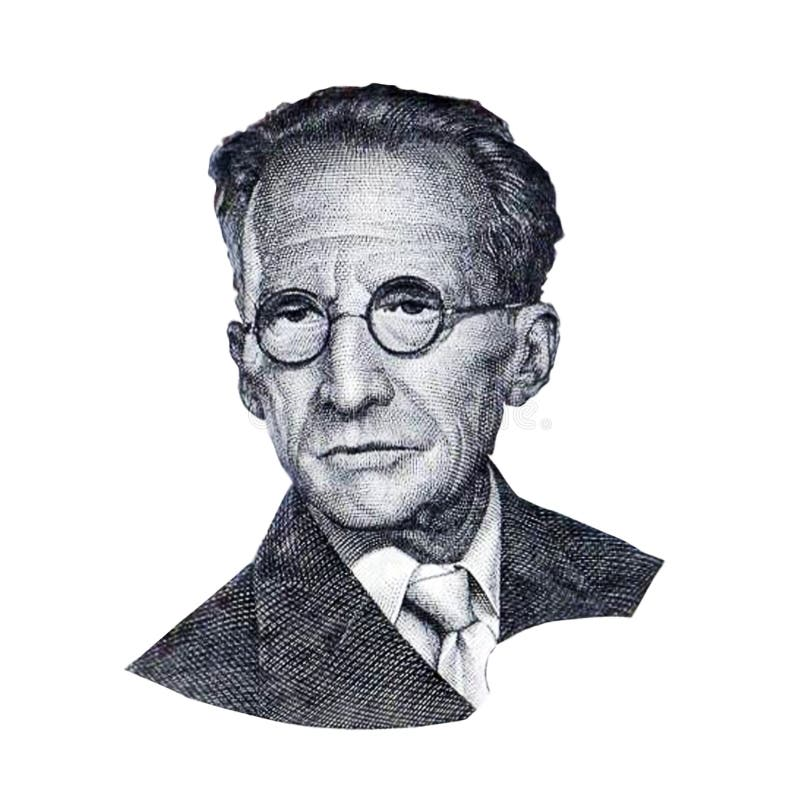
\includegraphics[width=0.6\textwidth]{image.png}}\\[\baselineskip]
  {\small\scshape University of Vienna}\par
  \vfill\null
\end{titlepage}

\section{The circuit model}
\subsection{Classical computation}
Use of classical computers (abstractly):

Solve problems $\equiv$ compute functions:
\begin{align*}
  f: \{0,1\}^n &\rightarrow \{0,1\}^m \\
  \underline{x}=(x_1,\ldots,x_n) &\mapsto f(x_1,\ldots,x_n)
\end{align*}

The \textbf{function $\bm{f}$} depends on the \textbf{problem} we want to solve, $\underline{x}$ encodes the \textbf{instance} of the problem.

\begin{example}
  Problem = \textbf{multiplication}: $(a,b)\mapsto a \cdot b$
  \begin{equation*}
    \underline{x}=(\underline{x}^1, \underline{x}^2) \mapsto f(\underline{x}) =\underline{x}^1 \cdot \underline{x}^2
  \end{equation*}

  Problem = \textbf{factorization}:
  \begin{equation*}
    \underline{x}: \text{ integer};\, f(\underline{x}): \text{ list of prime factors of (suitably encoded)}
  \end{equation*}
\end{example}

\paragraph{More precisely:} Each problem is encoded by a \textbf{family} of functions $f\equiv f^{(n)}:\{0,1\}^n\mapsto \{0,1\}^m$, with $m = \underbrace{\poly(n)}_{\mathclap{\text{\textbf{i.e.:} $m$ grows at most polynomially with $n$ (technically, }\exists \alpha > 0 \text{ s.th. }\frac{m}{n^\alpha}\rightarrow0).}},\,n \in \mathbb{N}$ -- one for each input size.

(Technical point: It must be possible to \emph{construct the functions $f^{(n)}$ systematically and efficiently}, see later!)

\textbf{Which ingredients} do we need to compute a \textbf{general function $\bm{f}$}?

\begin{enumerate}[label=(\roman*)]
  \item
    \begin{align*}
      f: \{0,1\}^n &\rightarrow \{0,1\}^m \\
      f(\underline{x}) &= (f_1(\underline{x}),\ldots,f_m(\underline{x}))\\
    \end{align*}
    where $f_k(\underline{x}): \{0,1\}^n \rightarrow \{0,1\}$

    $\Longrightarrow$ can restrict analysis to boolean functions
    \begin{equation*}
      f: \{0,1\}^n \rightarrow \{0,1\}.
    \end{equation*}

  \item Define $L=\{\underline{y} \mid f(\underline{y})=1\}=\{\underline{y}^1,\ldots, \underline{y}^l \}.$

    Define
    \begin{equation*}
      \underline{\delta}_{\underline{y}}(\underline{x})=
      \begin{cases}
        0 & \text{if } \underline{x}\neq \underline{y} \\
        1 & \text{if } \underline{x}=\underline{y}
      \end{cases}
    \end{equation*}

    Then, $f(\underline{x})=\underline{\delta}_{\underline{y}^1}(\underline{x}) \lor\underline{\delta}_{\underline{y}^2}(\underline{x}) \lor\ldots \lor \underline{\delta}_{\underline{y}^l}(\underline{x})$

  \item Define \textbf{bitwise} $\delta$:
    \begin{equation*}
      \delta_y(x)=
      \begin{cases}
        0 & \text{if } y\neq x \\
        1 & \text{if } y=x
      \end{cases}
    \end{equation*}

    Then
    \begin{equation*}
      \underline{\delta}_{\underline{y}}(\underline{x})=\delta_{y_1}(x_1)\land\delta_{y_2}(x_2)\land\ldots\land\delta_{y_n}(x_n)
    \end{equation*}

  \item
    \begin{equation*}
      \delta_y(x)=
      \begin{cases}
        x & \text{if } y=1 \\
        \lnot x & \text{if } y=0
      \end{cases}
    \end{equation*}
\end{enumerate}

\paragraph{Combine (i) - (iv):}

\textbf{Any $\bm{f(\underline{x})}$} can be constructed from \textbf{4 ingredients}: AND, OR and NOT gates, plus a COPY gate $x \mapsto (x,x)$.

This is called a \textbf{universal gate set}.

\begin{note}
  In fact, already either $\lnot (x \land y)$ NAND or $\lnot (x \lor y)$ NOR are universal, together with COPY.
\end{note}

This gives rise to the

\subsubsection*{Circuit model of computation}
The functions $f \equiv f^{(n)}$ which we can compute are construced by \textbf{concatening gates} from a simple \textbf{universal gate} set (e.g. AND, OR, NOT, COPY). \textbf{sequentially} in time (i.e., there are no loops allowed). This gives rise to a \textbf{circuit} for $f^{(n)}$.

The \textbf{difficulty} (\emph{computational hardness}) of a problem in the circuit model is measured by the number $K(n)$ of elementary gates needed to compute $f^{(n)}$ ($\hat{=}$ \# of time steps).

We often distinguish two qualitatively different regimes:
\begin{itemize}
  \item $K(n) \sim \poly(n)$: efficiently solvable (\textbf{class P}) \textbf{easy problems}
  \item $K(n) \gg \poly(n)$ -- e.g. $K(n) \sim \exp(n^\alpha)$: \textbf{hard problems}
\end{itemize}

\begin{note}[Technical]
  We must suppose that the circuits used for $f^{(n)}$ are \textbf{uniform}, i.e. they can be generated efficiently -- e.g. by a simple n-independent computer program. More formally, $f^{(n)}$ should be generated by a Turing machine.
\end{note}

\begin{example}
  \textbf{f = Multiplication}:

  Efficient:
  \begin{align*}
    &\underline{\overbrace{10110}^{l} \times \overbrace{10011}^{l'}} \\
    &10110\\
    &\phantom{101}10110\\
    &\underline{\phantom{1011}10110}\\
    &\underbrace{110100010}_{\mathclap{l \times l' \text{ additions: } \mathcal{O}(ll') \sim \mathcal{O}(n^2)\text{ gates}}}
  \end{align*}

  \textbf{f = Factorization}:

  \paragraph{E.g.:} Sieve of Eratosthenes:
  \begin{equation*}
    \{0,1\}^n \rightarrow \text{ try about }\sqrt{2^n} \sim 2^{\frac{n}{2}} \text{ cases}
  \end{equation*}
  $\Longrightarrow$ hard/exponential scaling

  No efficient algorithm known!
\end{example}

Is a \textbf{typical problem easy or hard}?
\begin{equation*}
  f: \{0,1\}^n \rightarrow \{0,1\}
\end{equation*}

Number of different $f$: $2^{(2^n)}$

\paragraph{But:} there are only $c^{\poly(n)}$ circuits of length $\poly(n)$ -- with $c$ denoting the number of elementary gates.

$\Longrightarrow$ As $n$ gets large, most f cannot be computed efficiently (i.e. with $\poly(n)$ operations).

Does the \textbf{computational power} depend on the \textbf{gate set}?

\textbf{NO!} By definition, any universal gate set can simulate any other gate set with constant overhead!

\begin{remark}
  There is a wide range of alternative models of computation, some more and some less realistic:
  \begin{itemize}
    \item CPU
    \item parallel computers
    \item \emph{Turing machines} -- tape + read/write head
    \item cellular automata
    \item \ldots and lots of exotic models \ldots
  \end{itemize}
\end{remark}

\textbf{But:} All known \emph{reasonable} models of computation can simulate each other with $\poly(n)$ overhead $\Longrightarrow$ same computational power (in the sense above).

\textbf{Church-Turing thesis:} All reasonable models of computation have the same computational power.

\subsection{Reversible circuits}
For quantum computing -- coming soon -- we will use the circuit model.
\begin{center}
  \textbf{Gates} will be replace by \textbf{unitaries}
\end{center}

\textbf{But:} Unitaries are \textbf{reversible} while \textbf{classical gates} (AND, OR) are \textbf{irreversible}.

Could such a model even do classical computations -- i.e., can we find a universal gate set with only reversible gates?

\textbf{YES!} -- \textbf{Classical computation} can be \textbf{made reversible}:

\paragraph{Toffoli gate:}
\begin{center}
  \begin{quantikz}
    \lstick{$x$} & \ctrl{1} & \rstick{$x$} \\
    \lstick{$y$} & \ctrl{1} & \rstick{$y$} \\
    \lstick{$z$} & \targ{} & \rstick{$z \oplus xy$}
  \end{quantikz}
  \bigskip
\end{center}
\begin{itemize}[label=$\rightarrow$]
  \item Toffoli gate is reversible (it is its own reverse, since $(z \oplus xy) \oplus xy = z$)
  \item Toffoli gate can simulate AND/OR/NOT/COPY, by using ancillas in state \emph{0} or \emph{1}:
\end{itemize}
\paragraph{E.g.:}
\begin{center}
  \centering
  \begin{minipage}{0.4\textwidth}
    \centering
    \begin{quantikz}
      \lstick{$x$} & \ctrl{1} & \rstick{$x$} \\
      \lstick{$1$} & \ctrl{1} & \rstick{$1$} \\
      \lstick{$0$} & \targ{} & \rstick{$x$}
    \end{quantikz}

    \textbf{COPY}
  \end{minipage}
  \begin{minipage}{0.4\textwidth}
    \centering
    \begin{quantikz}
      \lstick{$x$} & \ctrl{1} & \rstick{$x$} \\
      \lstick{$y$} & \ctrl{1} & \rstick{$y$} \\
      \lstick{$1$} & \targ{} & \rstick{$1\oplus(xy)=\lnot(xy)$}
    \end{quantikz}

    \textbf{NAND}
  \end{minipage}
  \bigskip
\end{center}

$\Longrightarrow$ gives reversible universal gate set (but requires ancillas).

This can be used to \textbf{compute any $\bm{f(\underline{x})}$ reversibly}, using ancillas, with essentially the same number of gates:
\begin{equation*}
  f^{\textnormal{R}}(\underline{x},\underline{y}) = (\underline{x},f(\underline{x}) \oplus \underline{y})
\end{equation*}

\emph{Idea.} Replace any gate by a reversible gate using ancillas. Then \emph{XOR} the result into $\underline{y}$ register. Finally, run the circuit backwards to \emph{uncompute} the ancillas. Ancilla count can be optimised for $\rightarrow$ cf. Preskill's notes

$\Longrightarrow$ Everything can be \textbf{computed reversibly}.

\textbf{BUT}: \textbf{3-bit} gate is \textbf{required}!

\subsection{Quantum Circuits}
Most common model for quantum computation:

\paragraph{The circuit model:}
\begin{itemize}
  \item Quantum system consisting of qubits: tensor product structure
  \item \textbf{Universal gate set} $S=\{U_1, \ldots U_k\}$ of few-qubit gates (typically 1- and 2-qubit gates) $U_j$. (See later for definition of \emph{universal}!)
  \item Construct circuits by sequentially applying elements of $S$ to a subset of qubits:
    \begin{equation*}
      \ket{\psi_{\textnormal{out}}} = V_T \ldots V_2 V_1 \ket{\psi_{\textnormal{in}}}
    \end{equation*}
    where $V_j$ are $U_j$ acting on a subset of qubits.

  \item Initial state:
    \begin{align*}
      \ket{\psi_{\textnormal{in}}} &= \ket{x_1}\ket{x_2}\ldots\ket{x_n}\overbrace{\ket{0}\ket{0}\ldots \ket{0}}^l \\
      &= \underbrace{\ket{\underline{x}}}_{\mathllap{\text{encodes instance of problem}}}\underbrace{\ket{\underline{0}}}_{\mathclap{\text{ancillas}}}
    \end{align*}
    \begin{itemize}
      \item alternatively, we can also have
        \begin{equation*}
          \ket{\psi_{\textnormal{in}}} = \ket{\underline{0}}\equiv\ket{0}^{\otimes l}
        \end{equation*}
        and encode the instance in the circuit.
    \end{itemize}
  \item At the end of the computation, measure the final state $\ket{\psi_{\textnormal{out}}}$ in the computational basis $\{\ket{0},\ket{1}\}$

    $\longrightarrow$ outcome $\ket{\underline{y}}$ with probability $p(y)=|\braket{\underline{y}|\psi_{\textnormal{out}}}|^2$
\end{itemize}

\emph{Notes:}

\begin{itemize}
  \item This is a \textbf{probabilistic} scheme -- it outputs $\underline{y}$ with some probability $p(\underline{y})$. In principle, we should compare to \textbf{classical probabilistic} schemes -- see later.
  \item We need not measure all qubits -- not measuring = trancing = measuring and ignoring outcome
  \item POVMs don't help -- we can simulate them (Naimark). Similarly, CP maps don't help -- we can simulate them (Stinespring + trace ancilla).
  \item Measurements at earlier times don't help: Can always postpone them (they commute). If gate at later time would depend on measurement outcome: This dependence can be realized \textbf{inside} the circuit with \emph{controlled gates}. (cf. later + homework)
\end{itemize}

What gate set should we choose?
\begin{itemize}
  \item There is a \textbf{continuum} of gates -- situation much more rich.
  \item \textbf{Different notions of universality} exist:
    \begin{itemize}
      \item \textbf{exact universality}: Any $n$-qubit gate can be realized \textbf{exactly}.
        $\longrightarrow$ Requires a \textbf{continuous family} of universal gates (counting argument!).
      \item \textbf{approximate universality}: Any $n$-qubit gate can be approximated well be gate set (finite gate set sufficient;\\
        \textbf{Solovan-Kitaev theorem:} $\varepsilon$-approximation (in $\norm{\cdot}_\infty$-Norm) of 1-qubit gate requires $\mathcal{O}(\poly(\log(1/\varepsilon)))$ gates from a suitable finite set.)
    \end{itemize}
  \item 1- and 2-qubit gates alone are universal! (cf. classical: 3-bit gates needed!)
  \item For \textbf{approximate universality}, \textbf{almost any} (with probability 1) \textbf{\emph{single} two-qubit gate} will do!
  \item More universal sets: later!
\end{itemize}

\subsection{Universal gate set}
Our \textbf{exact universal gate set}:
\begin{enumerate}[label=(\roman*)]
  \item 1-qubit rotations about X and Z axis:
    \begin{align*}
      R_x(\phi) &= e^{-i\phi \frac{X}{2}};\; X=
      \begin{pmatrix} 0 & 1 \\ 1 & 0
      \end{pmatrix},\, X^2=I \\
      R_z(\phi) &= e^{-i\phi \frac{Z}{2}};\; Z=
      \begin{pmatrix} 1 & 0 \\ 0 & -1
      \end{pmatrix},\, Z^2=I
    \end{align*}
    For $M^2=I$: $e^{-iM\frac{\phi}{2}}=\cos\frac{\phi}{2}I-i\sin\frac{\phi}{2}M$
    \begin{align*}
      \Longrightarrow R_x(\phi) &=
      \begin{pmatrix}
        \cos\frac{\phi}{2} & -i\sin\frac{\phi}{2} \\
        -i\sin\frac{\phi}{2} & \cos\frac{\phi}{2}
      \end{pmatrix}\\
      R_z(\phi) &=
      \begin{pmatrix}
        e^{-i\frac{\phi}{2}} & 0 \\
        0 & e^{i\frac{\phi}{2}}
      \end{pmatrix}
    \end{align*}

    Can be understood as rotations on Bloch sphere about X and Z axis by angle $\phi$ (i.e., rotations in $\textnormal{SO}(3)\cong \textnormal{SU}(2)/\mathbb{Z}_2$).

    Together, $R_x$ and $R_z$ generate all rotations in $\textnormal{SO}(3)$ (Euler angles!), and thus in $\textnormal{SU}(2)$ up to a phase.

    \begin{lemma}
      For any $U\in \textnormal{SU}(2)$,
      \begin{equation*}
        U=e^{i\phi}R_x(\alpha)R_z(\beta)R_x(\gamma) \quad \textnormal{for some } \phi,\alpha,\beta,\gamma.
      \end{equation*}
    \end{lemma}
    \begin{proof}
      Homework.
    \end{proof}
  \item \textbf{one} two qubit gate (almost all would do!). Typically, we use \emph{controlled-}NOT = CNOT:
    \begin{center}
      CNOT =
      \begin{quantikz}
        \lstick{$x$} & \ctrl{1} & \rstick{$x$} \\
        \lstick{$y$} & \targ{} & \rstick{$x\oplus y$}
      \end{quantikz}
      = $
      \begin{pmatrix} 1 & 0 & 0 & 0 \\ 0 & 1 & 0 & 0 \\ 0 & 0 & 0 & 1 \\ 0 & 0 & 1 & 0
      \end{pmatrix}$
    \end{center}
    CNOT flips $y$ iff $x=1$: \textbf{classical} gate!

    \textbf{Can prove}: This gate set can create \textbf{any} n-qubit $U$ \textbf{exactly} (but of course not efficiently -- $U$ has $\sim(n^n)^2=4^n$ real parameters).
\end{enumerate}

\subsubsection*{Overview of a number of important gates and identities}
\paragraph{Hadamard gate}:

\begin{equation*}
  H=\frac{1}{\sqrt{2}}
  \begin{pmatrix}
    1 & 1 \\ 1 & -1
  \end{pmatrix};\quad H=H^\dagger;\quad H^2=I.
\end{equation*}
\begin{align*}
  HR_x(\phi)H &= R_z(\phi) \\
  HR_z(\phi)H &= R_x(\phi) \\
\end{align*}
Graphical \emph{circuit} notation:
\begin{center}
  \begin{quantikz}
    &\gate{H} & \gate{X} & \gate{H}&
  \end{quantikz}
  =
  \begin{quantikz}
    &\gate{Z} &
  \end{quantikz}
  \bigskip
\end{center}

\emph{Important.} Matrix notation: time goes right to left. \\Circuit notation: time goes left to right.

\begin{center}
  \begin{quantikz}
    && \targ{} &&\\
    &\gate{H} & \ctrl{-1} & \gate{H} &
  \end{quantikz}
  =
  \begin{quantikz}
    & \ctrl{1} & \\
    & \ctrl{0} &
  \end{quantikz}
  =
  $
  \begin{pmatrix}
    1 & 0 & 0 & 0 \\
    0 & 1 & 0 & 0 \\
    0 & 0 & 1 & 0 \\
    0 & 0 & 0 & -1
  \end{pmatrix}$

  \emph{controlled-Z}, \emph{controlled-Phase}, CZ, CPHASE
  \bigskip
\end{center}

\begin{center}
  \begin{quantikz}
    & \gate{H} & \ctrl{1} & \gate{H} & \\
    & \gate{H} & \targ{} & \gate{H} &
  \end{quantikz}
  =
  \begin{quantikz}
    & \ctrl{1} & \\
    & \targ{} &
  \end{quantikz}
  \bigskip
\end{center}

\paragraph{Generally:} For a unitary $U \in \textnormal{SU}(2)$
\begin{center}
  \begin{quantikz}
    & \ctrl{1} & \\
    & \gate{U} &
  \end{quantikz}
  =
  $\left(
    \begin{array}{@{}c|c@{}}
      I & 0 \\
      \hline
      0 & U
  \end{array}\right)$

  \emph{controlled-U}
  \bigskip
\end{center}
Can be implemented with 2 CNOT (homework).

Also for $U \in \textnormal{SU}(2^n)$:

\begin{center}
  \begin{quantikz}[wire types={q,b}, classical
    gap=0.07cm]
    & \ctrl{1} & \\
    \lstick{$n$ \{}& \gate{U} &
    \end{quantikz}
    =
    $\left(
      \begin{array}{@{}c|c@{}}
        I_{2^n} & 0 \\
        \hline
        0 & U
    \end{array}\right)$
    \bigskip
  \end{center}

  \paragraph{Circuit for Toffoli:}
  \begin{center}
    \begin{quantikz}
      & \ctrl{1} &\\
      & \ctrl{1} &\\
      & \targ{} &
    \end{quantikz}
    =
    \begin{quantikz}
      && \ctrl{1} && \ctrl{1} & \ctrl{2} &\\
      &\ctrl{1}&\targ{} & \ctrl{1} & \targ{} &&\\
      & \gate{V} & & \gate{V^\dagger} & & \gate{V} &
    \end{quantikz}

    with $V=\frac{1-i}{2}(I+iX)$
    \bigskip
  \end{center}

  \paragraph{\emph{U} to controlled-\emph{U}:}
  Given circuit for $U$ -- in particular, a classical reversible circuit -- we can also build controlled-$U$:

  Just replace every gate by its controlled version, in particular Toffoli by

  \begin{center}
    \begin{quantikz}
      \lstick{$x$} & \ctrl{1} & \rstick{$x$}\\
      \lstick{$y$} & \ctrl{1} & \rstick{$y$}\\
      \lstick{$z$} & \ctrl{1} & \rstick{$z$}\\
      \lstick{$w$} & \targ{}  & \rstick{$w\oplus x \cdot y \cdot z$}
    \end{quantikz}
    \quad
    \begin{minipage}{0.4\textwidth}
      Toffoli with 3 controls: can be built from normal Toffoli (since classically universal!)
    \end{minipage}
    \bigskip
  \end{center}

  Finally, some \textbf{further approximate universal gate sets}:
  \begin{itemize}
    \item CNOT + 2 random 1-qubit gates
    \item CNOT + $H$ + $T = R_z(\frac{\pi}{4})$ \qquad (\emph{$\mathit{\frac{\pi}{8}}$ gate})
  \end{itemize}

  \section{Oracle-based algorithms}
  \subsection{The Deutsch algorithm}
  Consider $f:\{0,1\}^n\rightarrow\{0,1\}$. Let $f$ be \emph{very hard to compute} - e.g. long circuit.

  Want to know: Is $f(0)=f(1)$? (e.g.: will a specific chess move affect result?)

  How often do we have to run the circuit for $f$ (= \emph{evaluate f})? -- We think of $f$ as a \emph{black box} or \emph{oracle}: How many \textbf{oracle queries} are needed?

  \textbf{Classically}, we clearly need \textbf{2 queries}:
  \begin{equation*}
    \text{Compute } f(0) \text{ and } f(1).
  \end{equation*}
  Can quantum physics help?

  Consider \textbf{reversible implementation} of $f$:
  \begin{equation*}
    f^{\mathnormal{R}}:(x,y)\mapsto(x,y \oplus f(x))
  \end{equation*}
  \begin{center}
    \begin{quantikz}
      \lstick{$x$} & \gate[2]{U_f} & \rstick{$x$} \\
      \lstick{$y$} & \qw & \rstick{$y\oplus f(x)$}
    \end{quantikz}
    \quad
    $\ket{x}\ket{y}\mapsto \ket{x}\ket{y \oplus f(x)}$
    \bigskip
  \end{center}
  Of course, we can use $U_f$ to compute $f(0)$ or $f(1)$ on a quantum computer, but this we could also do classically. So, can we do better than this?

  Try to \textbf{use superposition as inputs}?

  \paragraph{First attempt:}
  \begin{center}
    \begin{quantikz}
      \lstick{$\frac{\ket{0}+\ket{1}}{\sqrt{2}}$} & \gate[2]{U_f} & \\
      \lstick{$\ket{0}$} &&
    \end{quantikz}
    $\equiv$
    \begin{quantikz}
      \lstick{$\ket{0}$} & \gate{H} & \gate[2]{U_f} & \\
      \lstick{$\ket{0}$} & & &
    \end{quantikz}
    \bigskip
  \end{center}
  \begin{equation*}
    \frac{\ket{0}+\ket{1}}{\sqrt{2}} \otimes \ket{0} = \frac{1}{\sqrt{2}} (\ket{0}\ket{0}+\ket{1}\ket{0})\xmapsto{U_f}\boxed{\frac{1}{\sqrt{2}} (\ket{0}\ket{f(0)}+\ket{1}\ket{f(1)})}
  \end{equation*}
  $\longrightarrow$ Have evaluated $f$ on \textbf{both outputs}!

  But how can we \textbf{extract the relevant information} from this state (i.e. do a \textbf{measurement})?

  \begin{itemize}
    \item Measure in computational basis: \textbf{collapse} superposition to \textbf{one case}!
    \item More generally: If $\bm{f(0) \neq f(1)}$, the output is in
      \begin{equation*}
        S_{\neq} = \left\{1/\sqrt{2}(\ket{00}+\ket{11}),1/\sqrt{2}(\ket{01}+\ket{10})\right\},
      \end{equation*}
      and for $\bm{f(0) = f(1)}$ in
      \begin{equation*}
        S_{=} = \{\ket{+}\ket{0},\ket{-}\ket{1}\}.
      \end{equation*}
      $\Longrightarrow$ not orthogonal, i.e. not (deterministically) distinguishable!

      But: We can do measurements which, with some probability, allows to conclude that $f(0)=f(1)$ or $f(0)\neq f(1)$. E.g., all states in $S_=$ are orthogonal to {$R_{\neq} = \{\ket{+}\ket{0},\ket{+}\ket{1}\}$}, and all states in {$S_{\neq}$} to { $R_{=}=\left\{\frac{\ket{00}-\ket{11}}{\sqrt{2}},\frac{\ket{01}-\ket{10}}{\sqrt{2}}\right\}$}.

      $\Longrightarrow$ A \textbf{POVM} which includes those outcomes plus an extra \emph{fail} outcome allows to unambiguously identify whether $f(0)\overset{?}{=}f(1)$ with some probability.

      Optimal success probability: $\frac{1}{2}$ (homework)

      While this is impossible classically, it does not give an improvement on average.
  \end{itemize}

  \paragraph{Second attempt:}
  \begin{center}
    \begin{quantikz}
      \lstick{$\ket{x}$} & \gate[2]{U_f} & \\
      \lstick{$\frac{\ket{0}-\ket{1}}{\sqrt{2}}$} &&
    \end{quantikz}
    $\equiv$
    \begin{quantikz}
      \lstick{$\ket{x}$} & & \gate[2]{U_f} & \\
      \lstick{$\ket{1}$} & \gate{H} & &
    \end{quantikz}
    \bigskip
  \end{center}
  \begin{align*}
    \ket{x}\left(\frac{\ket{0}-\ket{1}}{\sqrt{2}}\right)&\xmapsto{U_f}\ket{x}\left(\frac{\ket{f(x)}-\ket{1\oplus f(x)}}{\sqrt{2}}\right)\\[\parskip]
    &=
    \begin{cases}
      \ket{x}\left(\frac{\ket{0}-\ket{1}}{\sqrt{2}}\right) & \text{if } f(x)=0 \\[\parskip]
      \ket{x}\left(\frac{\ket{1}-\ket{0}}{\sqrt{2}}\right) & \text{if } f(x)=1
    \end{cases}\\[\parskip]
    &= \ket{x}\left[(-1)^{f(x)} \frac{\ket{0}-\ket{1}}{\sqrt{2}} \right] = (-1)^{f(x)}\ket{x}\left(\frac{\ket{0}-\ket{1}}{\sqrt{2}}\right)
  \end{align*}

  Not useful by itself: $f(x)$ only encoded in \textbf{global phase} for each \textbf{classical input} $\ket{x}$

  \paragraph{Combine attempts:}
  \begin{center}
    \begin{quantikz}
      \lstick{$\frac{\ket{0}+\ket{1}}{\sqrt{2}}$} & \gate[2]{U_f} & \\
      \lstick{$\frac{\ket{0}-\ket{1}}{\sqrt{2}}$} &&
    \end{quantikz}
    :
    \bigskip
  \end{center}
  \begin{align*}
    \frac{\ket{0}+\ket{1}}{\sqrt{2}}\otimes\frac{\ket{0}-\ket{1}}{\sqrt{2}} &= \frac{1}{\sqrt{2}}\left(\ket{0}\frac{\ket{0}-\ket{1}}{\sqrt{2}}+\ket{1}\frac{\ket{0}-\ket{1}}{\sqrt{2}}\right)\\[\parskip]
    &\xmapsto{U_f} \frac{1}{\sqrt{2}}\left((-1)^{f(0)}\ket{0}\frac{\ket{0}-\ket{1}}{\sqrt{2}}+(-1)^{f(1)}\ket{1}\frac{\ket{0}-\ket{1}}{\sqrt{2}}\right)\\[\parskip]
    &= \frac{(-1)^{f(0)}\ket{0}+(-1)^{f(1)}\ket{1}}{\sqrt{2}} \otimes \frac{\ket{0}-\ket{1}}{\sqrt{2}}
  \end{align*}

  \paragraph{Observations:}

  \begin{itemize}[label=$\rightarrow$]
    \item No entanglement created!
    \item 2nd qubit -- the one where $U_f$ outputs the fuction value -- is unchanged!!
    \item 1st qubit gets a phase $(-1)^{f(x)}$

      \centering \textbf{\emph{(phase kick-back technique)}}
  \end{itemize}

  \paragraph{State of 1st qubit:}
  \begin{align*}
    f(0)=f(1) &\Longleftrightarrow \frac{\ket{0}+\ket{1}}{\sqrt{2}}\\
    f(0)\neq f(1) &\Longleftrightarrow \frac{\ket{0}-\ket{1}}{\sqrt{2}}
  \end{align*}
  \begin{center}
    (up to irrelevant global phase)
  \end{center}

  \paragraph{Orthogonal states!} $\Longrightarrow$ measurement of 1st qubit in basis $\{\ket{+},\ket{-}\}$ (or apply
    \begin{quantikz}&\gate{H}&
  \end{quantikz} and measure in computational basis) allows to decide if $f(0) \overset{?}{=} f(1)$!

  \paragraph{Deutsch algorithm:}

  \begin{center}
    \begin{quantikz}
      \lstick{$\ket{0}$} & \gate{H} & \gate[2]{U_f} & \gate{H} & \meter{}&\setwiretype{c}\rstick{output $i=0,1$} \\
      \lstick{$\ket{1}$} & \gate{H} & & & &&
    \end{quantikz}
    \bigskip
  \end{center}

  \begin{align*}
    \text{output }i=0 &\Longrightarrow f(0)=f(1) \\
    i=1 &\Longrightarrow f(0)\neq f(1)
  \end{align*}

  \textbf{One application} of $U_f$ has been sufficient!

  $\Longrightarrow$ Speed-up compared to \textbf{classical algorithm} (1 vs. 2 oracle queries).

  \emph{Interesting to note:} 2nd qubit never needs to be measured -- and it contains \textbf{no information}.

  \paragraph{Two main insights:}
  \begin{itemize}
    \item Use input $\sum \ket{x}$ to \textbf{evaluate \emph{f} on all inputs simultaneously}.
    \item This parallelism alone is not enough -- \textbf{need a smart way to read out the relevant information}.
  \end{itemize}
  Howeverm a constant speed-up is not that impressive -- in particular, it is highly architecture-dependent!

  \textbf{Thus:}
  \subsection{The Deutsch-Josza algorithm}
  Consider $f:\{0,1\}^n\rightarrow\{0,1\}$ with \textbf{promise} (i.e., a condition we know is met by $f$) that
  \begin{align*}
    &\text{\textbf{either} } f(\underline{x}) = c \quad \forall \underline{x} \qquad &\text{\emph{(f constant)}}\\
    &\text{\textbf{or} } |\set{\underline{x}|f(\underline{x})=0}|=|\set{\underline{x}|f(\underline{x})=1}| \qquad &\text{\emph{(f balanced)}}
  \end{align*}

  \paragraph{Want to know:} Is f \textbf{constant} or \textbf{balanced}?
  \begin{center}
    How many queries are needed?
  \end{center}

  \paragraph{Use same idea:} Input $\sum \ket{x}$ and $\frac{\ket{0}-\ket{1}}{\sqrt{2}}$

  \begin{center}
    \begin{quantikz}[wire types={q,n,q,q}]
      \lstick[3]{n qubits} \ \ket{0}\ & \gate{H} \slice{$\scriptstyle\frac{1}{\sqrt{2^n}}\sum \ket{\underline{x}}\otimes \ket{-}$} & \gate[4]{U_f}&\gate{H}&\meter{}&\setwiretype{c} \ y_1\ \rstick[5]{\hspace{2em}output}\\
      & \vdots && \vdots\\
      \ \ket{0}\ &\gate{H}&&\gate{H}&\meter{}&\setwiretype{c} \ y_n\ \\
      \ \ket{1}\ &\gate{H}&&&
    \end{quantikz}
  \end{center}
  \begin{equation*}
    U_f: \ket{\underline{x}}\ket{y} \mapsto \ket{\underline{x}}\ket{y \oplus f(\underline{x})}
  \end{equation*}

  Before analyzing circuit:  What is \textbf{action of} $\bm{H^{\otimes n}}$?
  \begin{equation*}
    H:\; \ket{x} \mapsto \frac{1}{\sqrt{2}} \sum_{y=0,1} (-1)^{xy} \ket{y}
  \end{equation*}
  \begin{align*}
    H^{\otimes n}:\;\ket{x_1,\ldots,x_n} &\mapsto \frac{1}{\sqrt{2^n}} \sum_{\underline{y}} (-1)^{x_1y_1} \cdots (-1)^{x_ny_n} \ket{y_1,\ldots,y_n}\\
    \text{\textbf{or}:}\quad \ket{\underline{x}} &\mapsto \frac{1}{\sqrt{2^n}} \sum_{\underline{y}} (-1)^{\underline{x}\cdot\underline{y}} \ket{\underline{y}}
  \end{align*}
  where $\underline{x}\cdot\underline{y} = x_1y_1\oplus\ldots\oplus x_ny_n$
  \begin{center}
    \small
    (\enquote{scalar product} mod 2, \textbf{NOT} a scalar product!)
  \end{center}

  \paragraph{Analysis of circuit:} {\small(we omit normalization)}
  \begin{align*}
    \ket{\underline{0}}\ket{1} &\xmapsto{H^{\otimes n}\otimes H} \left(\sum_{\underline{x}}\ket{\underline{x}}\right)(\ket{0}-\ket{1})\\
    &\xmapsto{U_f} \left(\sum_{\underline{x}}(-1)^{f(\underline{x})}\ket{\underline{x}}\right)(\ket{0}-\ket{1})\\
    &\xmapsto{H^{\otimes n}\otimes I} \Biggl(\sum_{\underline{y}}\underbrace{\sum_{\underline{x}}(-1)^{f(\underline{x})+\underline{x}\cdot \underline{y}}}_{\eqcolon a_{\underline{y}}}\ket{\underline{y}}\Biggr)(\ket{0}-\ket{1})\\
  \end{align*}
  $p_y\coloneq |a_{\underline{y}}|^2$ is the probability to measure $\underline{y}=(y_1, \ldots, y_n)$.

  \paragraph{{\emph{f} constant:}} $f(\underline{x})=c$
  \begin{equation*}
    a_{\underline{y}} = (-1)^{c}\underbrace{\sum_{\underline{x}}(-1)^{\underline{x}\cdot \underline{y}}}_{\propto \; \delta_{\underline{y}, \underline{0}}} = (-1)^{c}\,\delta_{\underline{y},\underline{0}}
  \end{equation*}

  \paragraph{{\emph{f} balanced:}} $|\set{\underline{x}|f(\underline{x})=0}|=|\set{\underline{x}|f(\underline{x})=1}|$

  For $\underline{y}=\underline{0}$:
  \begin{equation*}
    a_{\underline{0}} = \sum_{\underline{x}}(-1)^{f(\underline{x})+\underline{x}\cdot \underline{0}} = \sum_{\underline{x}}(-1)^{f(\underline{x})} \underset{\scriptscriptstyle f \text{ balanced}}{=} 0
  \end{equation*}

  \paragraph{Thus:}
  \begin{align*}
    \text{Output } \underline{y}=\underline{0} &\Longrightarrow f \text{ constant} \\
    \text{Output } \underline{y}\neq\underline{0} &\Longrightarrow f \text{ balanced}
  \end{align*}

  $\Longrightarrow$ We can \textbf{unambiguously distinguish} between the 2 cases with \textbf{one query to the oracle for \emph{f}}!

  What is the \textbf{speed-up vs. classical methods}?
  \begin{itemize}
    \item \textbf{Quantum}: 1 use of $f$
    \item \textbf{Classical}: Worst case, we have to determine $2^{n-1}+1$ values of $f$ to be sure! $\Longrightarrow$ \textbf{exponential vs. constant}!
    \item \textbf{But:} If we are ok to get right answer with very high proability $p=1-p_{\textnormal{error}}$, then for $k$ queries to $f$,
      \begin{equation*}
        p_{\textnormal{error}} \approx  \underbrace{\frac{1}{2^k}}_{\mathclap{\approx\text{ probability to get $k$ times the same result for balanced $f$, if $k \ll 2^n$}}}
      \end{equation*}
      \textbf{i.e.:} $k\sim\log(1/p_\textnormal{error})$.
    \item \textbf{Randomized classical}: Much smaller speed-up vs. randomized classical algorithms (even for exponentially small error, $k\sim n$ oracle calls are sufficient.)
  \end{itemize}

  \subsection{Simon's algorithm}
  \ldots will give us a true exponential speed-up (also relative to \textbf{randomized} classical algorithms) in terms of oracle queries.
  \paragraph{Oracle:} $f:\{0,1\}^n\rightarrow\{0,1\}^n$ with the \textbf{promise}:
  \begin{equation*}
    \exists \underline{a} \neq \underline{0} \text{ s.th. } f(\underline{x}) = f(\underline{y}) \text{ \textbf{exactly if} } \underline{y} = \underline{x} \oplus \underline{a}.
  \end{equation*}
  \begin{center}
    \small \emph{(hidden periodicity)}
  \end{center}
  \paragraph{Task:} Find $\underline{a}$ by querying $f$.
  \paragraph{Classical:} Need to query $f(\underline{x}_i)$ until pair $\underline{x}_i,\underline{x}_j$ with $f(\underline{x}_i)=f(\underline{x}_j)$ is found.

  Roughly: k queries $x_1,\ldots,x_k \rightarrow\; \sim k^2$ pairs, for each pair: $\Pr(f(\underline{x}_i)=f(\underline{x}_j))\approx 2^{-n}$

  $\Longrightarrow\; p_{\textnormal{success}} \sim k^2 2^{-n} \Longrightarrow \text{need } k \sim 2^{n/2}$ queries!

  \paragraph{Quantum algorithm:} (Simon's algorithm)
  \begin{enumerate}[label=(\roman*)]
    \item Start with $\frac{1}{\sqrt{2^n}}\sum_{\underline{x}}\ket{\underline{x}}=H^{\otimes n}\ket{\underline{0}}$
    \item Apply $U_f:\ket{x}\ket{y}\mapsto\ket{x}\ket{y\oplus f(x)}$
      \begin{equation*}
        \left(\frac{1}{\sqrt{2^n}}\sum_{\underline{x}}\ket{\underline{x}}_A\right)\ket{0}_B \xmapsto{U_f} \frac{1}{\sqrt{2^n}}\sum_{\underline{x}}\ket{\underline{x}}_A\ket{f(\underline{x})}_B
      \end{equation*}
    \item \textbf{Measure \emph{B}}. $\Longrightarrow$ Collapse onto \textbf{random} $f(\underline{x}_0)$ (and thus random $\underline{x}_0$).

      $\Longrightarrow$ Register A colapses onto
      \begin{equation*}
        \frac{1}{N} \sum_{\mathclap{\substack{\underline{x}:\\f(\underline{x})=f(\underline{x}_0)}}}\ket{\underline{x}} = \frac{1}{\sqrt{2}}(\ket{\underline{x}_0}+\ket{\underline{x}_0\oplus \underline{a}})
      \end{equation*}
      \begin{center}
        How can we \textbf{extract \emph{a}}?\\ \small
        (Measure in computational basis $\rightarrow$ collapse on random $\underline{x}_0$: useless)
      \end{center}
    \item Apply $H^{\otimes n}$ again:
      \begin{align*}
        H^{\otimes n} \left( \frac{1}{\sqrt{2}}(\ket{\underline{x}_0}+\ket{\underline{x}_0\oplus \underline{a}}) \right) \ket{\underline{y}}&= \frac{1}{\sqrt{2^{n+1}}}\sum_{\underline{y}}\underbrace{\left[(-1)^{\underline{x}_0\cdot \underline{y}}+(-1)^{(\underline{x}_0\oplus \underline{a})\cdot \underline{y}}\right]}_{\mathclap{\substack{\underline{a}\cdot \underline{y}=0\; \Rightarrow \; =2 \cdot (-1)^{\underline{x}_0\cdot \underline{y}}\\\underline{a}\cdot \underline{y}=1\; \Rightarrow \; =0}}}\ket{\underline{y}}\\
        &= \frac{1}{\sqrt{2^{n-1}}}\sum_{\underline{y}:\:\underline{a}\cdot \underline{y}=0}(-1)^{\underline{x}_0\cdot \underline{y}}\ket{\underline{y}}
      \end{align*}
    \item Measure in \textbf{computational basis}:

      $\Longrightarrow$ obtain \textbf{random \emph{\underline{y}}} s.th. $\underline{a} \cdot \underline{y}=0$.

      ($n-1$) linear independent vectors $\underline{y}_i$ (over $\mathbb{Z}_2$) s.th. $\underline{a}\cdot \underline{y}_i=0$ allow to determine $\underline{a}$. (solve linear system of equations -- e.g. Gaussian elimination).

      Space of linear dependent vectors of $k$ vectors grows as $2^k$.\\
      $\Longrightarrow$ $\mathcal{O}(1)$ chance to find randomly linear independent vector\\
      $\Longrightarrow$ $\mathcal{O}(n)$ random $\underline{y}$ are enough\\
      $\Longrightarrow$ $\bm{\mathcal{O}(n)}$ \textbf{oracle queries} are enough (on average)
  \end{enumerate}

  \begin{equation*}
    \left.
    \begin{array}{ll}
      \text{\textbf{Classical: }} 2^{cn} \text{ queries}\\
      \text{\textbf{Quantum: }} c'n \text{ queries}
  \end{array}\right\}\text{ \textbf{exponential speed-up!}}
\end{equation*}

\emph{Notes:}
\begin{itemize}
  \item We don't have to measure B -- we never use the outcome! (But: Derivation easier this way!)
  \item $H^{\otimes n}\;\hat{=}$ (discrete) Fourier transform on $\mathbb{Z}_2^{\times n}$ $\longrightarrow$ \textbf{period finding} via \textbf{Fourier transform}.
\end{itemize}

\section{The quantum Fourier transform, period finding, and Shor's factoring algorithm}

Can we go beyond Fourier transform on $\mathbb{Z}_2$ (to $\mathbb{Z}_N$, for $N\sim 2^n$)?
\begin{itemize}
  \item What is the right transformation?
  \item Can it be implemented efficiently?
  \item What is it good for?
\end{itemize}

\subsection{The quantum Fourier transform}

Discrete Fourier transform (FT) on $\mathbb{C}^N$:
\begin{align*}
  x&=(x_0,\ldots,x_{N-1}) \in \mathbb{C}^N \\
  y&=(y_0,\ldots,y_{N-1}) \in \mathbb{C}^N\\
  FT:\;\mathcal{F}:\;x &\mapsto y\; \text{ s.th }\; y_k = \frac{1}{\sqrt{N}}\sum_{j=0}^{N-1}x_je^{2\pi ijk/N}
\end{align*}
\begin{definition}[Quantum Fourier transform (QFT)]
  \begin{equation*}
    \boxed{\ket{j} \mapsto \frac{1}{\sqrt{N}}\sum_{k=0}^{N-1}e^{2\pi ijk/N}\ket{k}}
  \end{equation*}

\end{definition}
\emph{Observe:}
\begin{equation*}
  \sum_j x_j \ket{j} \xmapsto{QFT} \sum_{jk} x_j e^{2\pi ijk/N}\ket{k} = \sum_k y_k \ket{k}
\end{equation*}
\textbf{i.e.:} QFT acts as \textbf{discrete FT on amplitudes}!

\paragraph{Computational cost of classical FT:}
\begin{itemize}
  \item $\mathcal{O}(N^2)$ operations.
  \item $N \sim 2^n$ $\Longrightarrow$ exponential in number of bits in N.
  \item Fast Fourier transform (FFT): only $\mathcal{O}(N\log N)$ operations, bit \textbf{still exponential}!
  \item $\mathcal{O}(n)$ is lower bound: minimal time to even just \textbf{output} $y_k$!
\end{itemize}

\paragraph{Will see:} QFT can be implemented on a quantum state in $\mathcal{O}(n^2)$ steps.

\begin{center}
  $\Longrightarrow$ exponential speed-up!

  (But only useful if input is given as quantum state!)
\end{center}
\paragraph{Step I:}\textbf{Rewrite QFT in binary}
\begin{itemize}
  \item Consider case $N=2^n$.
  \item Write $j$ etc. in binary:
    \begin{equation*}
      j = j_1j_2j_3\ldots j_n = j_1 2^{n-1}+j_2 2^{n-2}+\ldots+j_n 2^0
    \end{equation*}
  \item \emph{Decimal} point notation:
    \begin{equation*}
      0.j_l j_{l+1} \ldots j_n = \frac{1}{2}j_l + \frac{1}{4}j_{l+1} + \ldots + \frac{1}{2^{n-l+1}}j_n
    \end{equation*}
\end{itemize}

Then
\begin{align*}
  \ket{j} &\mapsto \frac{1}{2^{n/2}} \sum_{k=0}^{2^n-1} e^{2\pi ij\overbrace{k/2^n}^{\mathclap{\scriptstyle =0.k_1 k_2\ldots k_n}}}\ket{k} \\
  &= \frac{1}{2^{n/2}} \sum_{k_1 = 0}^1 \ldots \sum_{k_n = 0}^1 e^{2 \pi i j (\sum_{l=1}^n k_l 2^{-l})} \ket{k_1, k_2, \ldots ,k_n}\\
  &= \frac{1}{2^{n/2}} \sum_{k_1 = 0}^1 \ldots \sum_{k_n = 0}^1 \left[\bigotimes_{l=1}^n (e^{2\pi i j k_l 2^{-l}} \ket{k_l})\right]\\
  &= \bigotimes_{l=1}^n \left[ \frac{1}{\sqrt{2}} \sum_{k_l = 0}^1 e^{2\pi i j k_l 2^{-l}} \ket{k_l} \right] \\
  &= \bigotimes_{l=1}^n \frac{1}{\sqrt{2}} \left[  \ket{0} +{e^{2\pi i j 2^{-l}}} \ket{1} \right]
\end{align*}

\emph{Auxiliary calculation:}
\begin{gather*}
  j\cdot 2^{-l} = \underbrace{j_1 j_2 \ldots j_{n-l}}_{\text{integer}}.j_{n-l+1}\ldots j_n \\
  e^{2\pi i (j \cdot 2^{-l})} = e^{2\pi i \cdot (\text{integer}\,+\, 0.j_{n-l+1}\ldots j_n)} = e^{2\pi i \cdot 0.j_{n-l+1}\ldots j_n}
\end{gather*}

\begin{align*}
  \cdots = \frac{\ket{0}+e^{2\pi i 0.j_n} \ket{1}}{\sqrt{2}} \otimes \frac{\ket{0}+e^{2\pi i 0.j_{n-1}j_n} \ket{1}}{\sqrt{2}} \otimes \ldots \otimes \frac{\ket{0}+e^{2\pi i 0.j_1j_2\ldots j_n} \ket{1}}{\sqrt{2}}
\end{align*}

\paragraph{Step II:} Implement this \textbf{as a circuit}. Consider first only \textbf{rightmost term}:

\begin{equation*}
  \frac{\ket{0}+e^{2\pi i \cdot 0.j_1j_2\ldots j_n} \ket{1}}{\sqrt{2}} = \frac{\ket{0}+e^{2\pi i j_1/2}\cdot e^{2\pi i j_2/4}\cdot e^{2\pi i j_3/8}\cdots \ket{1}}{\sqrt{2}}
\end{equation*}

\begin{center}
  \bigskip
  \begin{quantikz}[wire types={q,q,q,n}, align equals at = 2]
    \lstick{$\ket{j_1}$} & \gate{H} & \gate{R_1} & \gate{R_2} & \rstick{$\cdots$}\\
    \lstick{$\ket{j_2}$} &\ghost{H}&\ctrl{-1}&&\rstick{$\cdots$} \\
    \lstick{$\ket{j_3}$} &\ghost{H}&&\ctrl{-2}& \rstick{$\cdots$}\\
    \lstick{\vdots} &&&& \\
  \end{quantikz}
  \qquad$R_d =
  \begin{pmatrix}
    1 & 0 \\
    0 & e^{2\pi i\cdot2^{-(d+1)}}
  \end{pmatrix}$
\end{center}
\paragraph{Actions of gates:}
\begin{align*}
  H&:\ket{j_1} &&\mapsto \ket{0}+e^{2\pi i 0.j_1}\ket{1} \\
  \text{C-}R_1&: \left(\ket{0}+e^{2\pi i 0.j_1}\ket{1}\right)\ket{j_2} &&\mapsto \left(\ket{0}+e^{2\pi i 0.j_1j_2}\ket{1}\right) \ket{j_2} \\
  \text{C-}R_2&: \left(\ket{0}+e^{2\pi i 0.j_1j_2}\ket{1}\right)\ket{j_2}\ket{j_3} &&\mapsto \left(\ket{0}+e^{2\pi i 0.j_1j_2j_3}\ket{1}\right) \ket{j_2}\ket{j_3} \\
\end{align*}
\begin{center}
  \vspace{-2ex}
  and so on \ldots
  \bigskip
\end{center}
$\longrightarrow$ Outputs the $n$-th qubit of the QFT on 1st qubit.
\paragraph{Continue in this vein:}

\begin{center}
  \begin{adjustbox}{width=\textwidth}
    \begin{quantikz}[wire types={q,q,q,n}]
      \lstick{$\ket{j_1}$} & \gate{H} & \gate{R_1} & \gate{R_2} & \ \cdots\ & \gate{R_{n-1}} &&&&&&& \rstick{$\ket{0}+e^{2\pi i 0.j_1\ldots j_n}\ket{1}$} \\
      \lstick{$\ket{j_2}$} &\ghost{H}&\ctrl{-1}&&&&\gate{H} & \gate{R_1} & \ \cdots\ & \gate{R_{n-2}}&&&\rstick{$\ket{0}+e^{2\pi i 0.j_2j_3\ldots}\ket{1}$}\\
      \lstick{$\ket{j_3}$} &\ghost{H}&&\ctrl{-2}&&&&\ctrl{-1}&&& \ \cdots \ && \rstick{$\ket{0}+e^{2\pi i 0.j_3j_4\ldots}\ket{1}$} \\
      \lstick{\vdots} &\ghost{H}\\
      \lstick{$\ket{j_n}$}&&&&&\ctrl{-4}&&&&\ctrl{-3}&\ \cdots \ & \gate{H}&\rstick{$\ket{0}+e^{2\pi i 0.j_n\ldots}\ket{1}$}
    \end{quantikz}
  \end{adjustbox}
  \bigskip
\end{center}
\paragraph{Gate count:} $\frac{n(n+1)}{2}= \bm{\mathcal{O}(n^2)}$ \textbf{gates!}

\emph{Notes:}
\begin{itemize}
  \item Output qubits in \textbf{reverse order} (can re-order if needed: $n/2$ swaps).
  \item
    \begin{quantikz}[align equals at = 1.5]
      &\gate{R_d}&\\
      & \ctrl{-1}&
    \end{quantikz}
    =
    \begin{quantikz}[align equals at = 1.5]
      & \ctrl{1}&\\
      &\gate{R_d}&
    \end{quantikz}
    $\Longrightarrow$ can flip C-$R_d$ gates

    Then, \textbf{upper} line acts as \textbf{control} in computational basis.\\
    $\Longrightarrow$ If we \textbf{measure} directly after QFT in computational basis, we can measure \textbf{before} the C-$R_d$ gates and control them classically:

    \begin{center}
      \begin{quantikz}
        \lstick{$\ket{j_1}$} & \gate{H} & \meter{} & \ctrl[vertical wire = c]{1} \setwiretype{c} & \ctrl[vertical wire = c]{2}&&&&&&\\
        \lstick{$\ket{j_2}$} &&&\gate{R_1}&&\gate{H}&\meter{}&\ctrl[vertical wire = c]{1} \setwiretype{c} &&& \\
        \lstick{$\ket{j_3}$} &&&&\gate{R_2}&&&\gate{R_1}&\gate{H}&\meter{} &\setwiretype{c}\\
        \lstick{\vdots}\\
      \end{quantikz}

      Only \textbf{one-qubit gates} needed!!

      (\emph{Where is the quantum-ness?})

    \end{center}
\end{itemize}

\subsection{Period finding}

Application of QFT: Find period of a function? (cf. Simon's algorithm)

Consider a periodic function $f:\mathbb{N}\rightarrow \set{0,\ldots,M-1}$ such that $\exists r > 0$ with $f(x) = f(x+r)$, and $f(x) \neq f(y)$ otherwise.

On a computer, we can only compute $f$ on a trucated input,
\begin{equation*}
  f:\: \underbrace{\set{0,\ldots,N-1}}_{=\{0,1\}^n} \rightarrow \underbrace{\set{0,\ldots,M-1}}_{=\{0,1\}^m}
\end{equation*}

\begin{center}
  (In particular, the periodicity of $f$ is broken across the boundary, if we think of $f(x+r) \equiv f((x+r) \mod N)$)
\end{center}

Can we find $r$ better than classically? (i.e., with much less than $\sim r$ queries to $f$)

Chosse $n$ such that $2^n \underbrace{\gg}_{\mathclap{\text{will make this specific later}}}r$

\begin{note}
  Since we do not know $r$, we need to know some upper bound on $r$ -- e.g., we can use that $r < M$.
\end{note}

Implement $U_f$ in quantum computer as before:
\begin{equation*}
  U_f:\: \ket{x}_A\ket{y}_B \mapsto \ket{x}_A\ket{y \oplus f(x)}_B
\end{equation*}

\paragraph{Algorithm:}
\begin{enumerate}[label=(\arabic*)]
  \item Hadamard on $A$, then $U_f$:
    \begin{equation*}
      \frac{1}{2^{n/2}}\sum\ket{x}_A\ket{0}_B \xmapsto{U_f} \frac{1}{2^{n/2}}\sum\ket{x}_A\ket{f(x)}_B
    \end{equation*}
  \item Measure $B$ register. For result $\ket{f(x_0)}_B$, $A$ collapses to
    \begin{equation*}
      \frac{1}{\sqrt{k_0}}\sum_{k=0}^{k_0-1}\ket{x_0+kr}
    \end{equation*}
    -- here, $0\leq x_0 < r$ and $\frac{2^n}{r} - 1 < k_0 \leq \frac{2^n}{r}$.
  \item Apply QFT:
    \begin{align*}
      &\mapsto \frac{1}{2^{n/2}\sqrt{k_0}}\sum_{k=0}^{k_0-1}\sum_{l=0}^{2^n-1}e^{2\pi i(x_0+kr)l/2^n}\ket{l}_A\\
      &= \sum_{l=0}^{2^n-1} \underbrace{e^{2\pi i x_0 l/2^n} \underbrace{\sum_{k=0}^{k_0-1} \frac{1}{2^{n/2}\sqrt{k_0}} e^{2\pi i rkl/2^n}}_{\eqcolon \hat{a}_l}}_{\eqcolon a_l}\ket{l}_A
    \end{align*}
  \item Measure in computational basis:
    \begin{equation*}
      |\hat{a}_l|^2: \text{ probability to obtain outcome } l
    \end{equation*}
\end{enumerate}

\paragraph{Intuitively:} $\hat{a}_l \propto \sum_k e^{2\pi i \left(\frac{rkl}{2^n}\right)}$ peaked around points $l$ where $\frac{rl}{2^n}$ is a close to an integer!
\begin{center}
  ($\longrightarrow$ Will quantify this in a moment!)
\end{center}

\paragraph{Intuitive picture:}
\begin{center}
  (General features of Fourier transforms -- nothing quantum!)
\end{center}

\begin{center}
  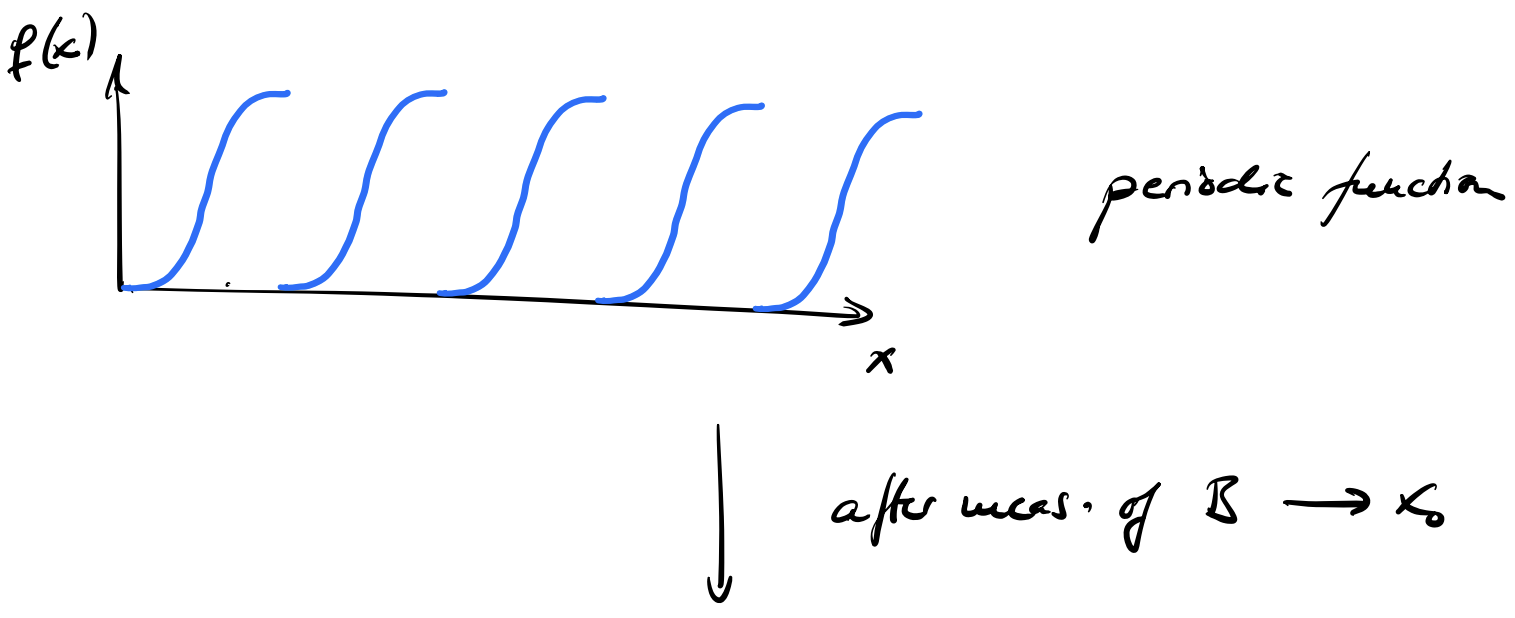
\includegraphics[width=0.8\textwidth]{image-3-1.png}\\
  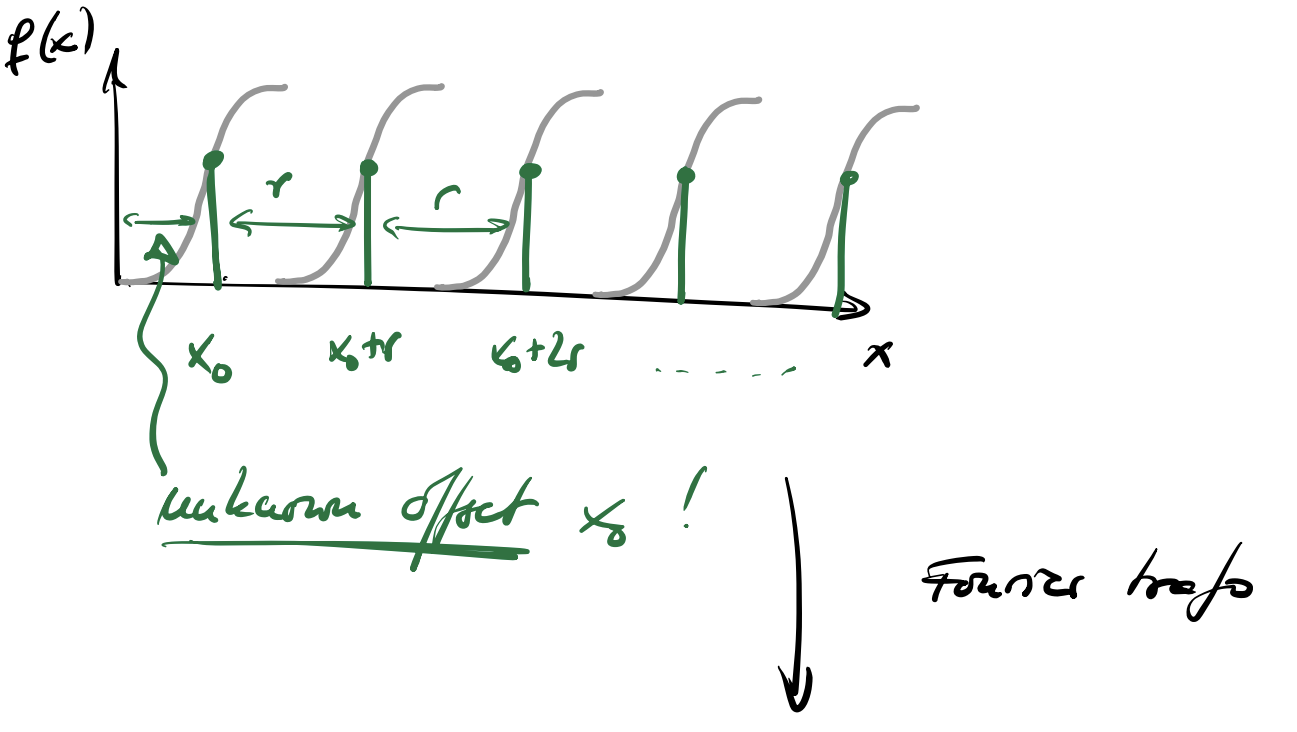
\includegraphics[width=0.8\textwidth]{image-3-2.png}\\
  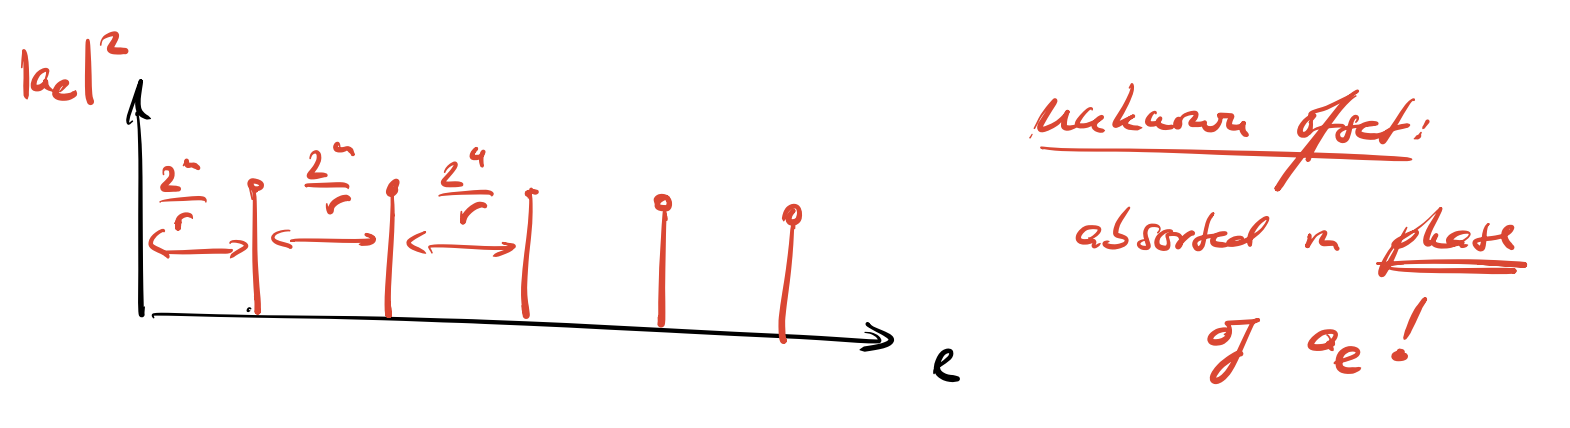
\includegraphics[width=0.8\textwidth]{image-3-3.png}
\end{center}

$\Longrightarrow$ can determine \textbf{multiple of $\bm{\frac{2n}{r}}$} by measuring $l$ (How to get $r$? Later!)

\paragraph{Detailed analysis of $\bm{|a_l|^2}$:}
How much \textbf{total weight} is in all $|a_l|^2$ with
\begin{equation*}
  l=\frac{2^n}{r}\cdot s + \delta+s;\; \delta_s \in \left(-\frac{1}{2}, \frac{1}{2}\right];\; s = 0,1,\ldots,r-1
\end{equation*}
\begin{center}
  (i.e. only those $l$ which are closest to $\frac{2^n}{r}\cdot s$)
\end{center}
\begin{align*}
  \text{Then, }\hat{a}_l &=\frac{1}{2^{n/2}\sqrt{k_0}}  \sum_{k=0}^{k_0-1} e^{2\pi i k\overbrace{(2+\frac{r}{2^n}\delta_s)}^{\equiv rl/2^n}} \\
  &= \frac{1}{2^{n/2}\sqrt{k_0}} \frac{e^{2\pi i \frac{r}{2^n}\delta_s k_0} - 1}{e^{2\pi i \frac{r}{2^n}\delta_s} - 1}\\[\parskip]
  \Aboxed{\text{\ldots since } \frac{2^n}{r}-1 &< k_0 \leq \frac{2^n}{r},\text{ and } r \ll 2^n:
  \frac{k_0 r}{2^n} = 1 - \varepsilon,\; 0 \leq \varepsilon \ll 1.}\\[\parskip]
  &= \frac{1}{2^{n/2}\sqrt{k_0}} \frac{e^{2\pi i \delta_s (1-\varepsilon)} - 1}{e^{2\pi i \frac{r}{2^n}\delta_s} - 1}\\[2\parskip]
  \Longrightarrow |\hat{a}_l|^2 &= \frac{1}{2^n k_0} \Big(\frac{\overbrace{|\sin(\pi \delta_s (1-\varepsilon))|}^{\mathclap{|\sin x|\geq \frac{|x|}{\pi/2}\text{ in relevant interval}}}}{\underbrace{|\sin(\frac{\pi r}{2^n} \delta_s)|}_{|\sin x| \leq |x|}}\Big)^2
  \geq \frac{1}{\cancel{2^n} k_0} \frac{\displaystyle \frac{\cancel{\pi ^2} \cancel{\delta_s^2} (1-\varepsilon)}{\pi^2/4}}{\displaystyle\frac{\cancel{\pi^2} r^2}{(2^n)^{\cancel{2}}}\cancel{\delta_s^2}}\\[\parskip]
  &= \frac{4}{\pi^2} \frac{1}{r} \frac{(1-\varepsilon)^2}{\frac{k_0 r}{2n}}= \frac{4}{\pi^2} \frac{1}{r} (1-\varepsilon) \approx \frac{4}{\pi^2}\frac{1}{r}
\end{align*}
\begin{center}
  (can be easily made more quantitatitve using $\varepsilon<\frac{r}{2^n}$!)
\end{center}

Since $s=0,1,\ldots,r-1$: Total probability that $|l-\frac{2^n}{r}s| \leq \frac{1}{2}$ for one such s: $p \geq \frac{4}{\pi^2} \approx 0.41$

With sufficiently high probability -- we will see that we can \textbf{check} success and thus repeat until we succeed! -- we obtain an $l$ s.th. $l=\frac{2^n}{r}s+\delta_s$, and thus,
\begin{equation*}
  \frac{l}{2^n} \approx \frac{s}{r},
\end{equation*}
where $s$ is chosen uniformly at random.

If we choose $r\ll2^n$ suitably, there is only \textbf{one} such ratio $\frac{s}{r}$ with $|l-\frac{2^n}{r}s| \leq \frac{1}{2}$, and it can be found efficiently. (see further reading.)

Specifically, it suffices to choose $N=2^n=(2^m)^2=M^2$, i.e. $m=2n$, and since $M\geq r:\; 2^n \gg 2^{n/2} > r.  $

If $s$ and $r$ are coprime, i.e. $\textnormal{gcd}(r,s)=1$, we can infer $r$ from $\frac{s}{r}$. This happens with probability at least $\Pr(\textnormal{gcd}(s,r)=1) \geq \frac{1}{\log r} \geq \frac{2}{\log 2}\cdot \frac{1}{n}$. (at least all primes $2\leq s < r$ are good, and density of primes is $\frac{1}{\log r}$)

$\Longrightarrow$ with $\mathcal{O}(n)$ iterations, we find a $s$ coprime with r.

Once we have used this to obtain a guess for $r$, we can \textbf{test} whether $f(x)=f(x+r)$, and repeat until success!

$\Longrightarrow$ Efficient algorithm for period finding; $\mathcal{O}(n)$ applications of $f$ required!

\subsection{Application: Factoring algorithm}

\paragraph{Factoring:} Given $N\in\mathbb{N}$ (not prime), find $f \in \mathbb{N},\, f\neq1,$ such that $f|N$.

(\emph{Note:} Primality of $N$ can be checked efficiently.)

This can be \textbf{solved efficiently} if we have an efficient method for \textbf{period finding}!

\subsubsection*{Sketch of algorithm}
\begin{enumerate}[label=(\arabic*)]
  \item Select a random $a$, $2\leq a<N$.
    \begin{equation*}
      \text{If } \underbrace{\textnormal{gcd}(a,N)}_{\mathclap{\text{efficiently computable!}}} > 1 \Longrightarrow \text{ done, } f=\textnormal{gcd}(a,N)!
    \end{equation*}
    \textbf{Thus:} Assume $\textnormal{gcd}(a,N)=1$.
  \item Denote by $r$ the smallest $x>0$ such that $a^x \mod N = 1$.
    -- that is, the period of $f_{N,a}(x)\coloneq a^x \mod N$.

    $r$ is called the \textbf{order of \emph{a} mod \emph{N}}.

    (\emph{Note:} Some $z>1$ s.th. $a^z \mod N = 1$ must exist since
      \begin{align*}
        \exists x,y &\in \set{1,\ldots,N}:\; a^x \equiv a^y \mod N \text{ (counting possibilities)}\\
        &\Longrightarrow a^x(1-a^{y-x}) \equiv 0 \mod N \Longrightarrow N|(a^x(1-a^{y-x})) \\
      &\xLongrightarrow{\scriptscriptstyle\textnormal{gcd}(a,N)=1} N|(1-a^{y-x}) \Longrightarrow a^{y-x} \equiv 1 \mod N\quad \qed \: )
    \end{align*}

    Furthermore, $f_{N,a}(x)$ can be \textbf{computed efficiently} (recall: \emph{Efficient} means \emph{polynomial in number of digits of $N$}):

    Using $x = x_{m-1}2^{m-1}+x_{m-2}2^{m-2}+\ldots$,
    \begin{equation*}
      a^x \mod N = {\underbrace{(a^{(2^{m-1})})}}^{x_{m-1}}\cdot (a^{(2^{m-2})})^{x_{m-2}}\cdot \ldots \mod N
    \end{equation*}
    \begin{center}
      Effeciently computable via reapeated squaring mod $N$:\\
      $a \mapsto a^2 \mod N \mapsto a^4 \mod N \mapsto \ldots$,\\
      by doing \enquote{mod $N$} at each step the numbers don't require an exponential number of digits:\\
      $\mathcal{O}(n)$ multiplications of $n$-digit numbers.
    \end{center}

    $\Longrightarrow$ $r$ can be \textbf{found efficiently} with a \textbf{quantum computer}!

  \item Assume for now \textbf{\emph{r} even}:
    \begin{equation*}
      a^r \mod N = 1 \Longleftrightarrow N|(a^r - 1) \Longleftrightarrow N|(a^{r/2}+1)(a^{r/2}-1)
    \end{equation*}
    However, we also know that $N \nmid a^{r/2}-1$, since otherwise $a^{r/2} \mod N = 1$ (contradiction)

    $\Longrightarrow$ \textbf{either} $N|(a^{r/2}+1)$ \textbf{or} $N$ has non-trivial common factors with \textbf{both} $a^{r/2} \pm 1$.
    \begin{align*}
      &\Longrightarrow 1 \neq f \coloneq \textnormal{gcd}(N,a^{r/2}+1) \nmid N\\
      &\Longrightarrow \text{ found a \textbf{non-trivial factor \emph{f} on \emph{N}!}}
    \end{align*}

    $\Longrightarrow$ Algorithm will succeed as long as
    \begin{enumerate}[label=(\roman*)]
      \item $r$ is even
      \item $N \nmid (a^{r/2}+1)$
    \end{enumerate}
    This can be shown to happen with probability $\geq \frac{1}{2}$ for a random choice of $a$ (see further reading).
    \begin{itemize}
      \item \textbf{unless} either $N$ is even (can be checked efficiently) \textbf{or} $N=p^k$ for some prime $p$ (can also be checked efficiently by taking roots; there are only $\mathcal{O}(\log N)$ roots which one has to check!)
      \item \textbf{and} in \textbf{both cases}, this gives a non-trivial factor!
    \end{itemize}
\end{enumerate}

$\Longrightarrow$ \textbf{Efficient Quantum Algorithm for Factoring.}

\begin{center}
  \textbf{\emph{Shor's Algorithm}}
\end{center}
\end{document}
